\documentclass[9pt,a4paper]{extarticle}
\usepackage[margin=1.8cm]{geometry}
\usepackage{titlesec}
\usepackage[british]{babel}
\usepackage{fontspec}
\setmainfont{Arial}[Path=/System/Library/Fonts/Supplemental/,Extension=.ttf,UprightFont=Arial,BoldFont=Arial Bold,ItalicFont=Arial Italic,BoldItalicFont=Arial Bold Italic]
\usepackage{graphicx}
\usepackage{booktabs}
\usepackage{tabularx}
\usepackage{float}
\usepackage{caption}
\usepackage{subcaption}
\usepackage[round]{natbib}
\usepackage[hidelinks]{hyperref}

\captionsetup{font=small, labelfont=bf, skip=3pt}
\graphicspath{{../figures/}}
\setlength{\parindent}{0pt}
\setlength{\parskip}{2pt}
\setlength{\intextsep}{3pt}
\titlespacing*{\section}{0pt}{0pt}{4pt}

\begin{document}

\section*{Part A: Preprocessing and EDA}
\renewcommand{\thefigure}{A\arabic{figure}}
\renewcommand{\thetable}{A\arabic{table}}
The seed is 32. Using this seed I shuffled each class of the training set once, then took the first 500 images as training and the next 50 as validation, so no image is in both. The test sample is 50 images per class from the test set, evaluated once at the end.

\textbf{A1 Data.} Each image is 32 × 32 pixels with three colour channels (values from 0 to 255). The average and spread of each channel in my training sample are within 0.002 of the full training set (Table~\ref{tab:a1}, Figure~\ref{fig:a1}).

\noindent
\begin{minipage}[c]{0.54\textwidth}
\centering\small
\captionof{table}{CIFAR-10 \citep{krizhevsky2009cifar} sizes; [0, 1] channel statistics.}
\label{tab:a1}
\begin{tabular}{@{}lrrr@{}}
\toprule
& Train & Test & My samples \\
& (full) & (full) & (train, val., test) \\
\midrule
Images & 50,000 & 10,000 & 5,000, 500, 500 \\
Per class & 5,000 & 1,000 & 500, 50, 50 \\
\bottomrule
\end{tabular}

\vspace{6pt}
\begin{tabular}{@{}lcc@{}}
\toprule
& Mean (R, G, B) & Std (R, G, B) \\
\midrule
Training sample & 0.491, 0.482, 0.445 & 0.247, 0.243, 0.261 \\
Full training & 0.491, 0.482, 0.447 & 0.247, 0.243, 0.262 \\
\bottomrule
\end{tabular}
\end{minipage}\hfill
\begin{minipage}[c]{0.42\textwidth}
\centering
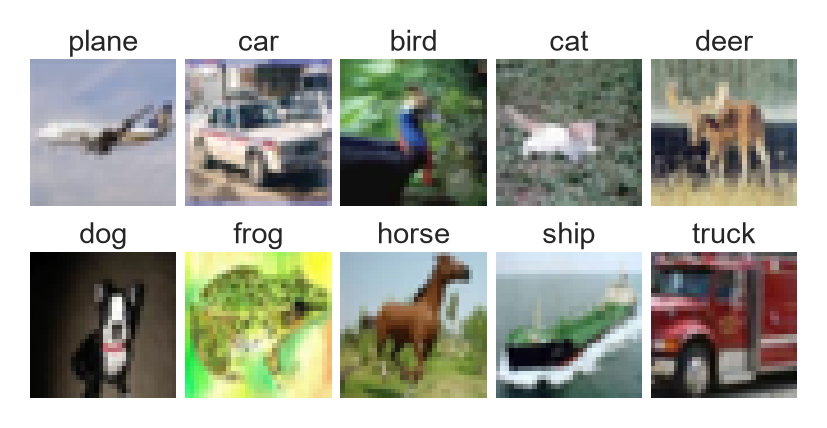
\includegraphics[width=\linewidth]{a1_examples.png}
\captionof{figure}{One training image per class; poses and positions vary.}
\label{fig:a1}
\end{minipage}
\vspace{4pt}

\textbf{A2 Data quality.} To find near-duplicates, I fitted PCA on the training sample (206 components, 95.0\% of the variance), projected all 60,000 images onto it and found the nearest neighbour of each. I scored each image by the ratio of its nearest to its second-nearest distance and counted a pair when the ratio was below 0.8 (\citealp{lowe2004sift}; Figure~\ref{fig:a2}a). A plain distance cut-off would not separate copies from other images. Some clear copies (ratio below 0.5) are as far apart as 5.79, while 4,628 images with a ratio of 0.9 or more sit closer than that. With the ratio, I found 1,028 pairs within training, 423 between training and test and 31 within test. The counts are approximate, because a photo with two copies has a ratio near 1. My samples hold 5 training-validation pairs below 0.8. A needless swap costs little, so A3 uses 0.85, which catches 7 training-validation and 1 training-test pair (Table~\ref{tab:a2}).

\emph{Poor quality.} For each image I measured brightness (mean grey level), contrast (standard deviation) and sharpness (log variance of a 3 × 3 Laplacian; \citealp{pechpacheco2000diatom}). I then took the modified z-score, built from the median and the median absolute deviation (MAD), and flagged an image if it was beyond ±3.5 \citep{iglewicz1993outliers}. This flagged 24 of 5,000 training images: 2 dark, 10 bright, 1 high contrast and 11 low sharpness. All are valid photos and none is constant (Figure~\ref{fig:a2}b).

\emph{Look-alike classes.} For each training image I looked at its 10 nearest neighbours. On average 77.1\% of them have a different label (90\% if neighbours were random), and 1,169 images have no neighbour from their own class. Deer makes up 19.3\% of all neighbours, which inflates the deer column of Figure~\ref{fig:a2}c (27.0\% of frog neighbours are deer). Lift divides each share by the neighbour class's overall share. Taking the smaller of the two directions, it was highest for automobile and truck (1.75), cat and dog (1.66) and airplane and ship (1.59).

\begin{figure}[H]
\centering
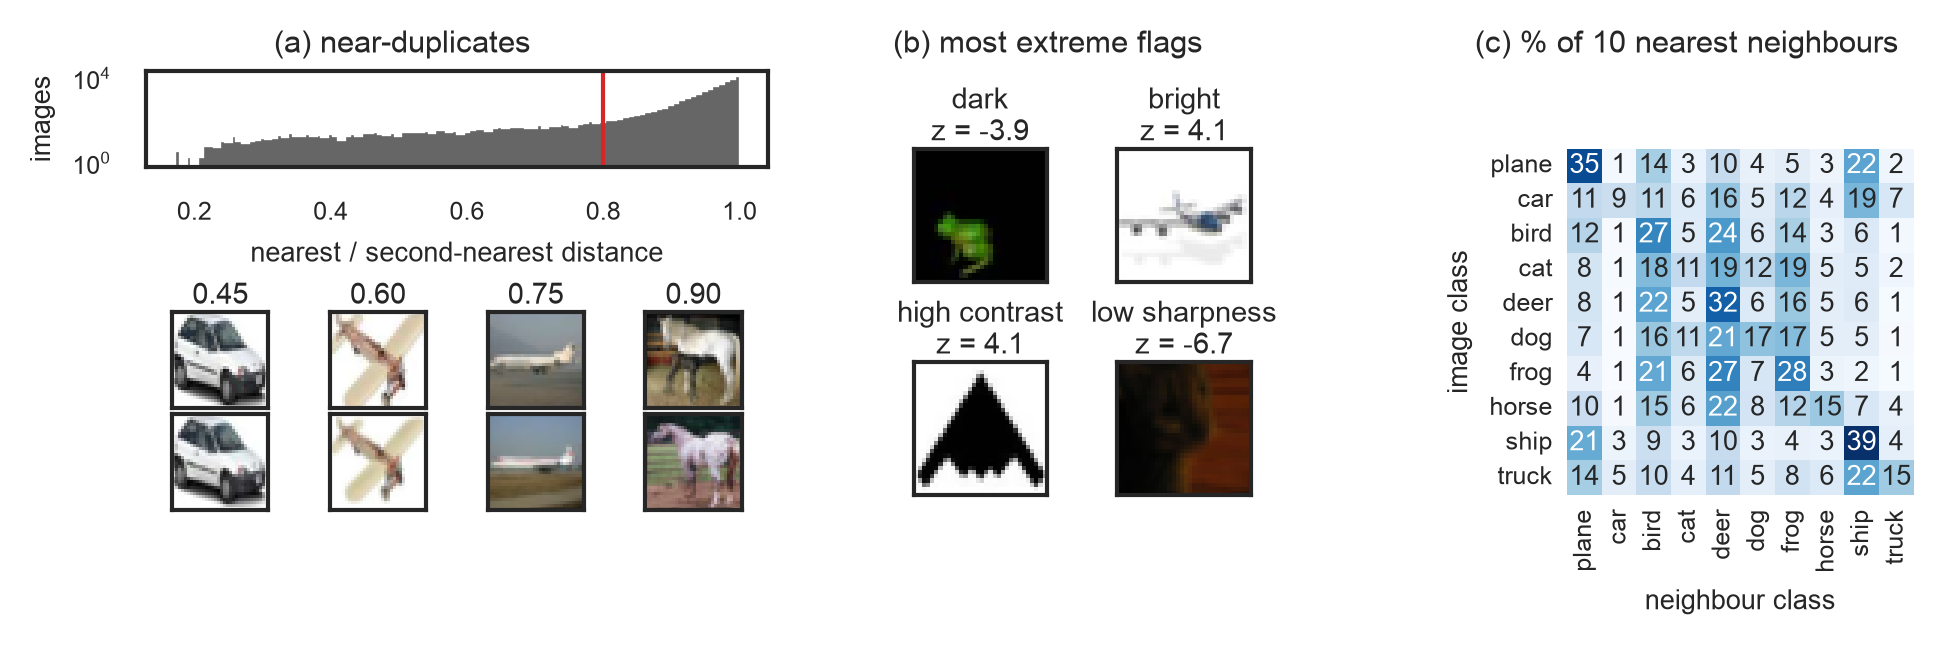
\includegraphics[width=0.92\textwidth]{a2_quality.png}
\caption{(a) Nearest to second-nearest distance ratio for all 60,000 images, cut-off 0.8 in red, with example pairs below. (b) Most extreme flags. (c) \% of each class's 10 nearest neighbours. Low ratios are the same photo; similar scenes can also fall below 0.8.}
\label{fig:a2}
\end{figure}

\begin{table}[H]
\centering\footnotesize\renewcommand{\arraystretch}{1.0}
\caption{A3 preprocessing pipeline. Step 1 uses test pixels only, never test labels.}
\label{tab:a2}
\begin{tabularx}{\textwidth}{@{}>{\raggedright\arraybackslash}p{0.42\textwidth}>{\raggedright\arraybackslash}p{0.25\textwidth}>{\raggedright\arraybackslash}X@{}}
\toprule
Step & Evidence & Reason \\
\midrule
1. Replace the 8 training images paired with validation or test images by unsampled same-class images (seed 33). & 7 training-validation, 1 training-test pair at 0.85; 0 after swaps (A2). & Copies inflate scores. 5 within-training pairs stay. \\
2. Keep ambiguous images and the 23 still flagged. & 0 constant; valid images (A2b). & Outliers are real data. \\
3. Normalise channels with the cleaned training mean (0.491, 0.482, 0.445) and std (0.247, 0.243, 0.261). & Raw means 0.445 to 0.491; validation means then 0.006 to 0.043. & Zero-centred inputs help gradient descent; fit on training only. \\
4. Part C training only: random flip and 32 × 32 crop after 4-pixel padding. & Objects face either way, off-centre (Figure~\ref{fig:a1}). & CNNs are shift-equivariant, not invariant. \\
\bottomrule
\end{tabularx}
\end{table}

\textbf{Reflection.} The ratio test found copies that a plain distance cut-off missed. I replaced the 8 training images that matched a validation or test image, to avoid leakage and the Part C model remembering them. I would also check the third-nearest image to catch photos with two copies. Many look-alike images seem to share a background, so I would predict that Part B pixel clusters group airplane with ship and frog with deer. If Part C confuses the same classes, this may be a sign that it is using the background.

\newpage
\section*{Part B: Unsupervised Learning}
\setcounter{figure}{0}\setcounter{table}{0}
\renewcommand{\thefigure}{B\arabic{figure}}
\renewcommand{\thetable}{B\arabic{table}}
\textbf{B1 Features and PCA.} I compared two ways of describing each image: the 3,072 normalised pixel values from A3, and 512 values from the layer before the classifier of ResNet-18 \citep{he2016resnet}. ResNet-18 was trained on ImageNet \citep{deng2009imagenet} and not fine-tuned on CIFAR-10. Images were resized to 224 × 224 with ImageNet normalisation. I standardised each feature on the 5,000 cleaned training images so that no feature dominates, then kept enough PCA components for 90\% of the variance: 100 for pixels and 193 for embeddings (Figure~\ref{fig:b1}). Keeping 95\% instead would need 210 and 274, so for pixels the last 5\% of variance costs more components than the first 90\%.

\begin{figure}[H]
\centering
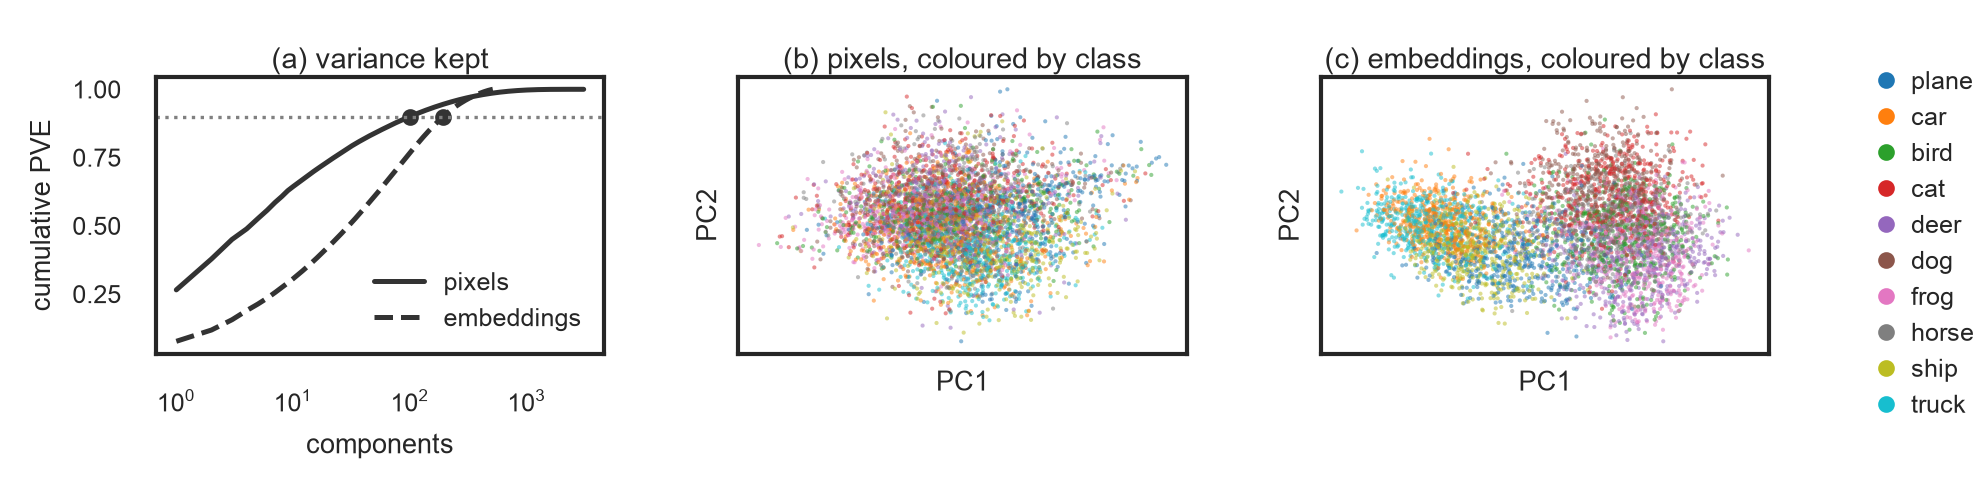
\includegraphics[width=0.92\textwidth]{b1_pca.png}
\caption{(a) Cumulative variance kept, 90\% dotted. (b, c) First two components by class. Only embeddings separate vehicles from animals.}
\label{fig:b1}
\end{figure}

\textbf{B2 Clustering and choosing k.} Using scikit-learn \citep{pedregosa2011sklearn}, I ran k-means (10 restarts) and Ward clustering on the PCA features of both feature sets, for \textit{k} from 2 to 20, without labels. Ward merges the two clusters whose union least increases the within-cluster variance \citep{ward1963}. The silhouette \citep{rousseeuw1987silhouette} scores how much closer each image is to its own cluster than to the next nearest one, from −1 to 1. Two clusters scored best in all four combinations, but for embeddings, four clusters came close (k-means 0.064 at \textit{k} = 2 against 0.051 at \textit{k} = 4; Figure~\ref{fig:b2}a). The best value, 0.163, is low, so the clusters overlap. The k-means elbow (the point furthest from a straight line joining the two ends of the curve) was 7 for pixels and 8 for embeddings, but the elbow was not sharp: the distance from that line was within 0.01 of its peak across \textit{k} = 6 to 8 for pixels and 6 to 10 for embeddings (Figure~\ref{fig:b2}b). So I used \textit{k} = 2 from the silhouette, and also ran \textit{k} = 10 to compare with the 10 classes.

\begin{figure}[H]
\centering
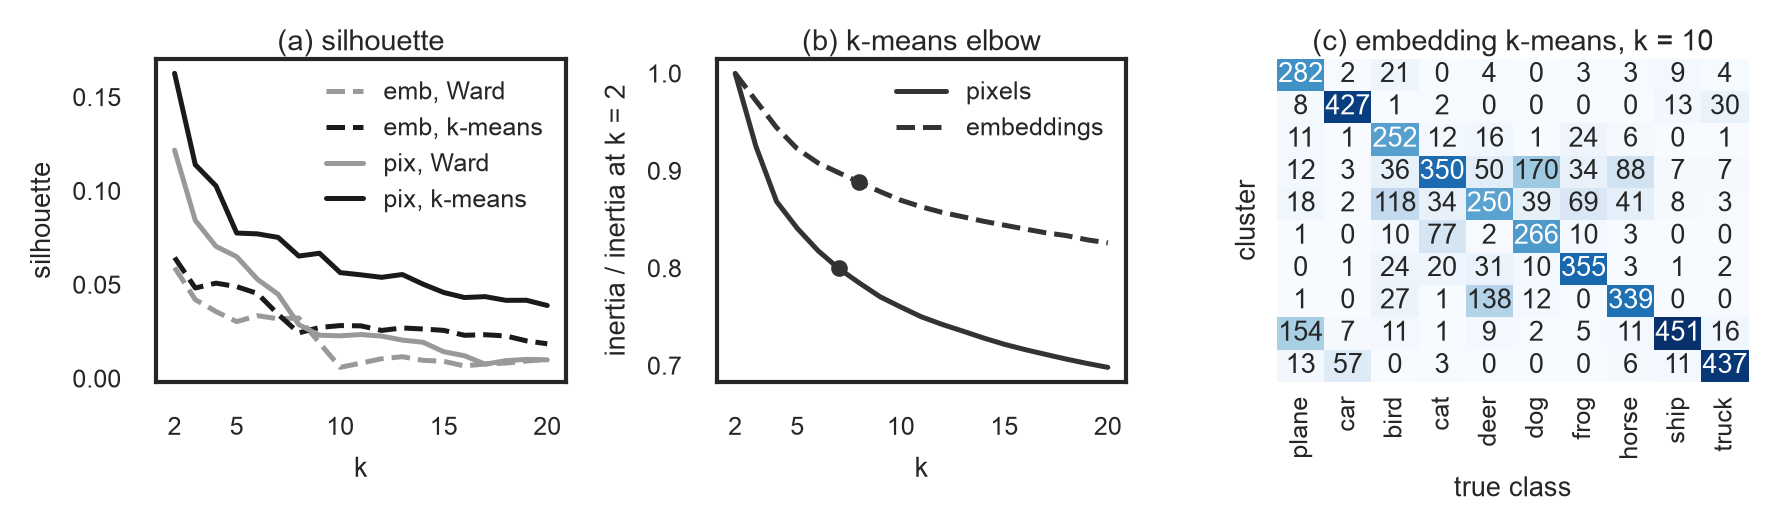
\includegraphics[width=0.97\textwidth]{b2_clusters.png}
\caption{(a) Silhouette. (b) K-means inertia relative to \textit{k} = 2. (c) Embedding k-means, \textit{k} = 10. Silhouette favours \textit{k} = 2; plane, car and truck clusters are purest.}
\label{fig:b2}
\end{figure}

\textbf{B3 Evaluation.} Here I used the labels to score the clusters with ARI \citep{hubert1985ari}, where 1 is a perfect match and 0 is chance (Table~\ref{tab:b1}). At \textit{k} = 2, embedding k-means split animals from vehicles with 95.1\% agreement, against 63.2\% for pixels. At \textit{k} = 10, embedding k-means matched the classes most closely, and Ward scored lower than k-means in every case. The silhouette preferred pixels (0.056 against 0.028), whereas ARI preferred embeddings (0.461 against 0.044), so a higher silhouette did not mean a closer match to the classes. Pixels follow brightness: pixel PC1 correlates 0.988 with mean brightness, and the pixel cluster of 149 ships and 93 airplanes is the second brightest. Another pixel cluster is led by deer and frogs (128 each), as Part A predicted. In the embedding clusters (Figure~\ref{fig:b2}c), cat and dog share two clusters, 154 airplanes fall in the ship cluster, and 138 deer fall in the horse cluster. The A2 pairs cat and dog, and airplane and ship, stay mixed, but automobile and truck separate. ImageNet contains many dogs, vehicles and ships, so these scores flatter the embeddings. Part C must learn shape cues that pixels lack, and should find cat and dog hardest, then airplane and ship.

\begin{table}[H]
\centering\footnotesize
\caption{Clustering scores; silhouette uses no labels. Purity is at most 0.2 at \textit{k} = 2. Embedding k-means at \textit{k} = 10 is closest to the classes.}
\label{tab:b1}
\begin{tabular}{@{}llrrrrrr@{}}
\toprule
& & \multicolumn{3}{c}{\textit{k} = 2} & \multicolumn{3}{c}{\textit{k} = 10} \\
\cmidrule(lr){3-5}\cmidrule(l){6-8}
Features & Method & Silhouette & Purity & ARI & Silhouette & Purity & ARI \\
\midrule
Pixels & K-means & 0.163 & 0.155 & 0.022 & 0.056 & 0.224 & 0.044 \\
Pixels & Ward & 0.122 & 0.140 & 0.010 & 0.023 & 0.216 & 0.038 \\
Embeddings & K-means & 0.064 & 0.198 & 0.151 & 0.028 & 0.682 & 0.461 \\
Embeddings & Ward & 0.059 & 0.196 & 0.150 & 0.006 & 0.577 & 0.357 \\
\bottomrule
\end{tabular}
\end{table}

\textbf{Reflection.} Embeddings recovered far more of the classes than pixels did (ARI 0.461 against 0.044). Even so, without labels the only clear split was animals against vehicles: the silhouette never passed 0.17, and the elbow was flat. Two things may have made this harder. Standardising gave features that barely vary the same weight as informative ones, which amplified their noise. K-means also expects round clusters of similar size, and real classes rarely look like that. Next, I would try DBSCAN, since it finds clusters of any shape and does not need \textit{k} to be chosen in advance.


\newpage
\section*{Part C: Neural Networks for Computer Vision}
\setcounter{figure}{0}\setcounter{table}{0}
\renewcommand{\thefigure}{C\arabic{figure}}
\renewcommand{\thetable}{C\arabic{table}}
\textbf{C1 Baseline and design.} For the baseline, I built a small CNN in PyTorch \citep{paszke2019pytorch} and trained it from random weights, with nothing pretrained. It has two blocks, each a 3 × 3 convolution with 32 filters and padding 1, followed by ReLU and 2 × 2 max pooling. The maps are then flattened and passed to a dense layer of 128 units with ReLU, and a final layer gives one score for each of the 10 classes. I trained it on the Part A pipeline without augmentation, using cross-entropy loss and Adam (learning rate 0.001, batch size 64), with gradients from backpropagation. I chose ReLU because sigmoid units make gradients vanish in deeper networks. The 3 × 3 filters keep the weight count low. With padding 1, the image stays 32 pixels wide, which follows from W\textsubscript{2} = (W\textsubscript{1} − F + 2P)/S + 1 with F = 3, P = 1 and S = 1. Max pooling then halves the width and makes the network less sensitive to small shifts, so the maps go from 32 × 32 × 32 to 32 × 16 × 16 and then 32 × 8 × 8. In total, the network has 273,706 parameters.

Every run uses 30 epochs and seed 32 unless stated, so runs are comparable. Each keeps the weights from the epoch with the lowest validation loss. For the baseline, this is epoch 6, where training accuracy is 0.656. After that, validation loss rises while training accuracy reaches 1.000 by epoch 23, so the baseline overfits (Figure~\ref{fig:c1}a, b).

\begin{figure}[H]
\centering
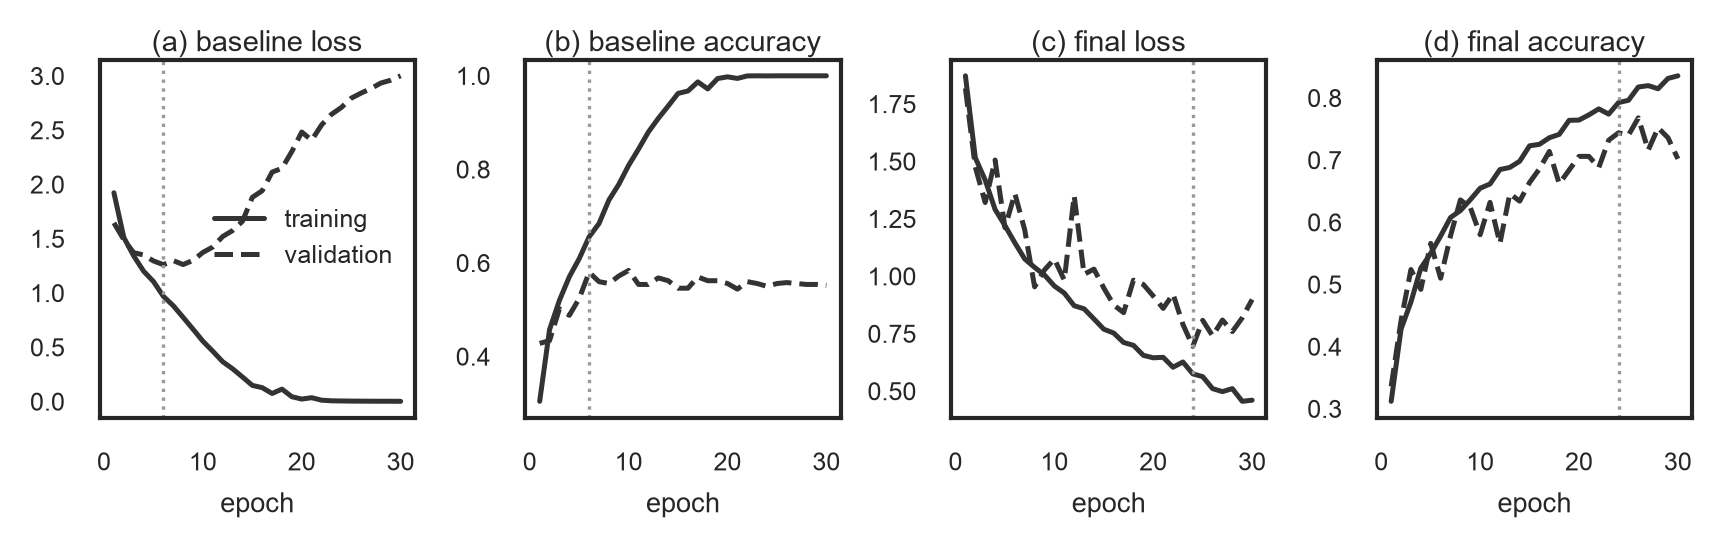
\includegraphics[width=\textwidth]{c1_curves.png}
\caption{Training and validation loss and accuracy for (a, b) the baseline and (c, d) the final model; dotted line at the lowest validation loss. The baseline overfits after epoch 6; the final model's validation loss falls, with noise, to its lowest at epoch 24.}
\label{fig:c1}
\end{figure}

\textbf{C2 Experiments.} I first added each change to the baseline on its own and compared them on validation (Table~\ref{tab:c1}). With only 500 validation images, an accuracy near 0.55 has a 95\% interval of ±0.044, so smaller differences could be chance. The baseline itself ranged from 0.528 to 0.580 across three seeds.

Only augmentation clearly helped, raising seed-32 accuracy from 0.580 to 0.666. Batch normalisation (0.570) stayed within the baseline's range, and dropout 0.3 (0.582) was only just above it. A deeper VGG-style net \citep{simonyan2015vgg}, with three blocks of two 3 × 3 convolutions (32, 64 and 128 filters), scored 0.556. It fitted the training set almost perfectly (0.992) but did no better on validation, so it overfitted.

Combined with augmentation, the deeper net gave 0.666, no better than augmentation alone, but adding batch normalisation raised it to 0.744. Depth only helped once batch normalisation was added. Adding dropout as well gave 0.722, but both augmented dropout runs peaked at epochs 28 and 30, so 30 epochs may have been too few to judge them.

The final model (Figure~\ref{fig:c1}c, d) is the best combination on seed 32: the deeper net with augmentation, and batch normalisation and ReLU after every convolution. Its maps shrink from 32 × 32 × 32 to 128 × 4 × 4, and it has 551,466 parameters. Retrained with seeds 33 and 34, which were not used to choose it, it scored 0.738 and 0.742, so its range (0.738 to 0.744) is clear of the baseline's. I compared ten configurations on the same 500 validation images, so 0.744 is probably a little high; the test set gives the fair figure.

\begin{table}[H]
\centering\footnotesize
\caption{Validation results, seed 32 unless three seeds are shown as mean (range). Best epoch has the lowest validation loss. Training accuracy is the running accuracy on training batches at epoch 30, with augmentation and dropout on where used.}
\label{tab:c1}
\begin{tabular}{@{}lrrrrr@{}}
\toprule
Change & Validation accuracy & Macro-F1 & Best epoch & s per epoch & Training accuracy \\
\midrule
Baseline (3 seeds) & 0.549 (0.528 to 0.580) & 0.547 & 6.3 & 0.581 & 1.000 \\
+ augmentation & 0.666 & 0.667 & 21 & 0.705 & 0.686 \\
+ batch norm & 0.570 & 0.569 & 5 & 0.904 & 0.923 \\
+ dropout 0.3 & 0.582 & 0.574 & 10 & 0.760 & 0.888 \\
+ deeper (VGG-style) & 0.556 & 0.554 & 10 & 1.543 & 0.992 \\
Aug + BN & 0.662 & 0.662 & 29 & 1.453 & 0.692 \\
Aug + BN + dropout & 0.656 & 0.656 & 30 & 1.426 & 0.574 \\
Aug + deeper & 0.666 & 0.663 & 22 & 1.706 & 0.754 \\
\textbf{Aug + BN + deeper (3 seeds)} & \textbf{0.741 (0.738 to 0.744)} & \textbf{0.739} & 24.3 & 2.059 & 0.839 \\
Aug + BN + dropout + deeper & 0.722 & 0.720 & 28 & 1.995 & 0.750 \\
\bottomrule
\end{tabular}
\end{table}

\textbf{C3 Final result.} I chose and froze the seed-32 final model before testing and ran it once on the 500 test images. It scored 0.746 accuracy (95\% interval ±0.038) and macro-F1 0.745, close to its 0.744 on validation.

\textbf{C4 Evaluation and interpretation.} Cat is the weakest class (F1 0.55) and ship the strongest (0.85; Table~\ref{tab:c2}). The confusion matrix (Figure~\ref{fig:c2}a) shows 22\% of cats called dogs and 22\% of dogs called cats. Next come trucks called cars (18\%), cars called trucks (12\%) and planes called ships (12\%), while only 4\% of ships were called planes.

Cat and dog link all three parts (Table~\ref{tab:c3}). They had a pixel lift of 1.66 in A2, shared an embedding cluster 32.6\% of the time in B3 against 6.0\% for an average pair, and are now the most confused pair. B3 predicted airplane and ship would come next, but car and truck did. They were the strongest pixel pair, and shared an embedding cluster only 15.1\% of the time, yet the CNN still confuses them, as pixels did. Deer and horse shared embedding clusters 24.7\% of the time, but the CNN rarely confuses them (4\%).

The most confident mistakes (Figure~\ref{fig:c2}b) include two horses on open fields called planes and a cat beside a zigzag pattern called a frog, which suggests background and texture drive some errors. For a correctly classified cat, two of the three strongest last-layer channels peak on the cat. For a cat called a dog, they fire in scattered patches (Figure~\ref{fig:c4}).

\begin{figure}[H]
\centering
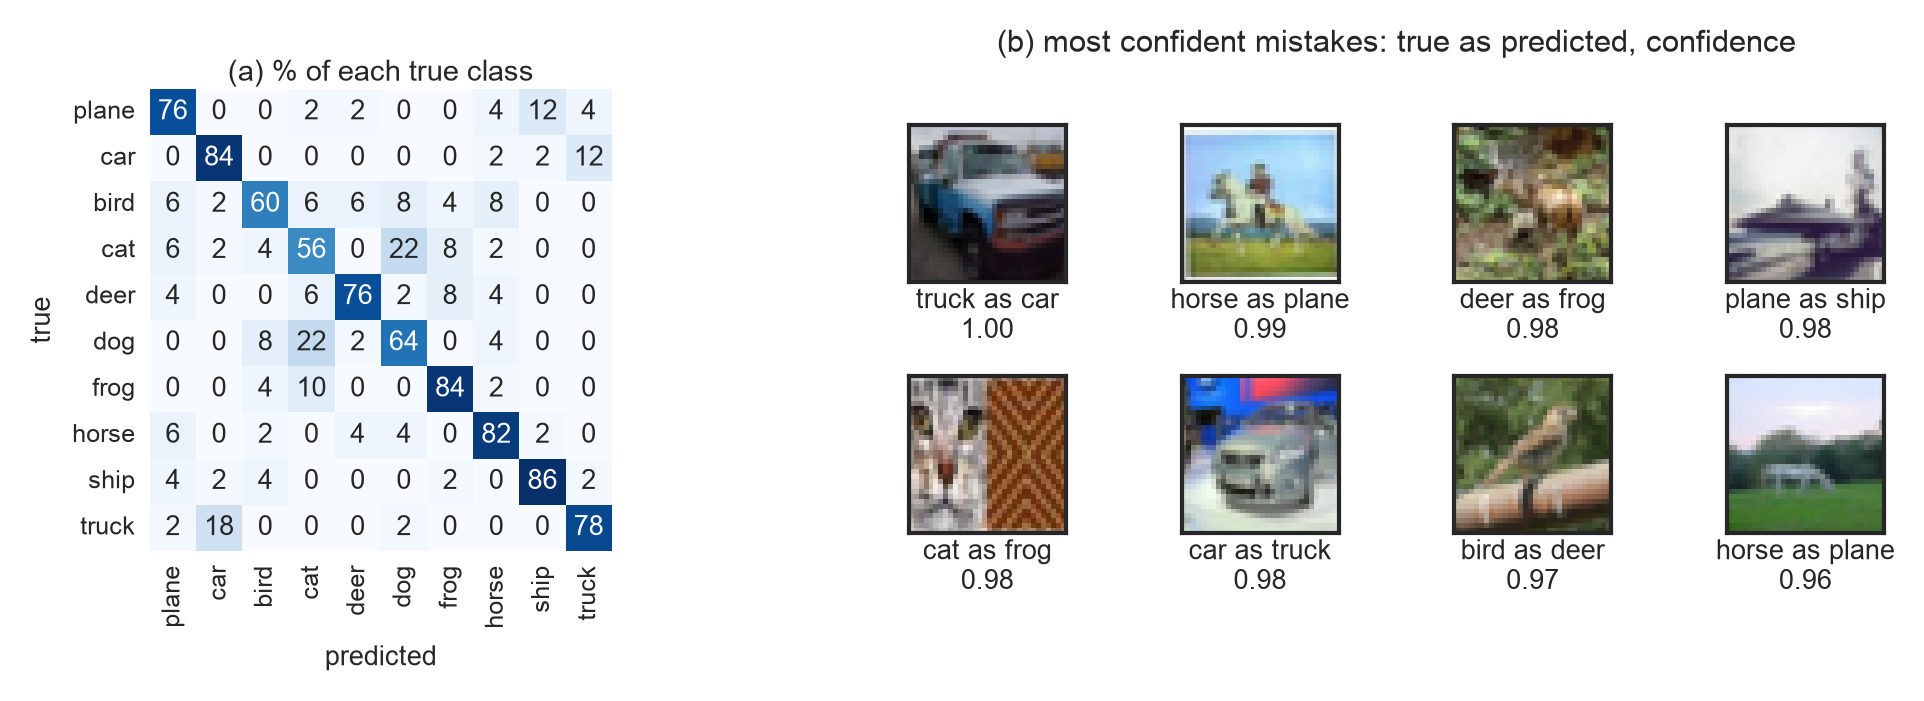
\includegraphics[width=\textwidth]{c2_confusion.png}
\caption{(a) Test confusion matrix, \% of each true class. (b) The eight most confident mistakes, true as predicted, with softmax confidence. Cat and dog are confused 22\% each way; several confident mistakes appear to share a background with the predicted class.}
\label{fig:c2}
\end{figure}

\begin{table}[H]
\centering\footnotesize
\caption{Per-class test results. Cat is weakest, ship strongest.}
\label{tab:c2}
\begin{tabular}{@{}lrrrrrrrrrr@{}}
\toprule
& plane & car & bird & cat & deer & dog & frog & horse & ship & truck \\
\midrule
Precision & 0.73 & 0.78 & 0.73 & 0.55 & 0.84 & 0.63 & 0.79 & 0.76 & 0.84 & 0.81 \\
Recall & 0.76 & 0.84 & 0.60 & 0.56 & 0.76 & 0.64 & 0.84 & 0.82 & 0.86 & 0.78 \\
F1 & 0.75 & 0.81 & 0.66 & 0.55 & 0.80 & 0.63 & 0.82 & 0.79 & 0.85 & 0.80 \\
\bottomrule
\end{tabular}
\end{table}

\begin{table}[H]
\centering\footnotesize
\caption{Look-alike pairs across Parts A, B and C: pixel lift (A2), share of image pairs in one embedding cluster (B3) and test confusion each way (C4). Cat and dog are high at every stage.}
\label{tab:c3}
\begin{tabular}{@{}lrrr@{}}
\toprule
Pair & A2 lift & B3 same cluster & C4 confused \\
\midrule
cat, dog & 1.66 & 0.326 & 0.22, 0.22 \\
plane, ship & 1.59 & 0.290 & 0.12, 0.04 \\
car, truck & 1.75 & 0.151 & 0.12, 0.18 \\
deer, horse & 0.91 & 0.247 & 0.04, 0.04 \\
average pair & & 0.060 & 0.028 \\
\bottomrule
\end{tabular}
\end{table}

\begin{figure}[H]
\centering
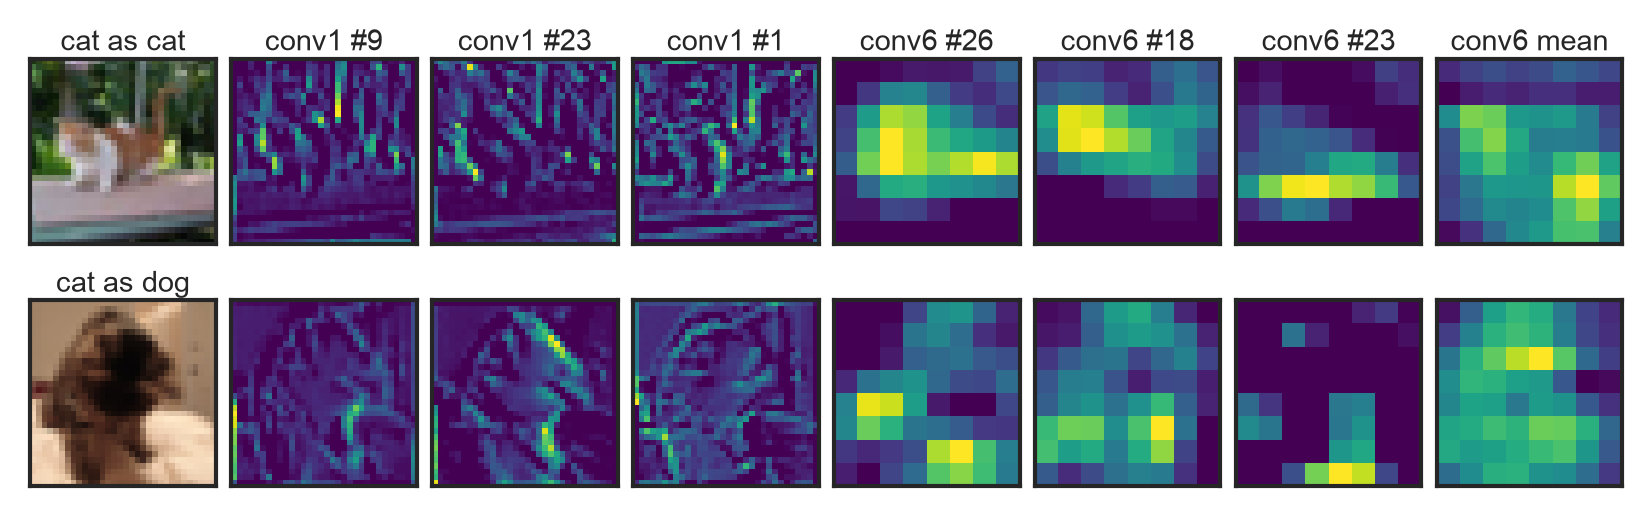
\includegraphics[width=\textwidth]{c4_feature_maps.png}
\caption{A correctly classified cat (top) and a cat predicted as dog (bottom): the three strongest first-layer and last-layer maps, and the last-layer mean. First-layer maps trace edges in both; on the misclassified cat the last layer fires in scattered patches. Each map has its own colour scale.}
\label{fig:c4}
\end{figure}

\textbf{Reflection.} Data was the biggest limit: with 5,000 training images, the baseline started overfitting after epoch 6. The test set is small too. Its accuracy is only known to within ±0.038, and each class has just 50 test images, so I would not read much into small gaps between classes. I also gave batch normalisation and dropout only one seed each on their own, which was too few runs to tell whether either one helps. Every run had the same 30 epochs, but the augmented dropout runs peaked at epochs 28 and 30, so a longer schedule might have changed which model won. For Part A, I would redo the duplicate search with my trained network's features instead of raw pixels. Two copies of a photo with different brightness or cropping look different as pixels but should look similar as features. For Part B, I would cluster those features too and compare them with ResNet-18's, to see whether a network trained only on CIFAR-10 learns the classes as well as one trained on ImageNet. Everything ran on my M2 MacBook Air through PyTorch's MPS backend. One epoch took 0.581 s for the baseline and 2.059 s for the final model, and all runs together took 9.2 minutes.

\newpage
\bibliographystyle{plainnat}
\bibliography{references}

\end{document}
